\documentclass{article}
\usepackage{graphicx}
\usepackage{geometry}
\usepackage[hidelinks]{hyperref}
\usepackage{rotating}
\usepackage{subcaption}
\usepackage{epstopdf}

% \usepackage{biblatex}

\geometry{
    a4paper,
    total={170mm,257mm},
    left=20mm,
    top=20mm,
}

% \bibliography{references}

\title{Single-cyclist crash classification guide}
\author{
  Benjam\'in Gonz\'alez\\
  \small{\href{mailto:b.gonzaleztoledo@tudelft.nl}{B.GonzalezToledo@tudelft.nl}}
  }
\date{\today}

\begin{document}

\maketitle

%\begin{sidewaysfigure}
%    \centering
%    \includegraphics[width = \textwidth]{class-mindmap-v3.png}
%    \caption{Flowchart of bicycle crash classification.}
%    \label{fig: flowchart}
%\end{sidewaysfigure}

%\begin{figure}
%    \centering
%    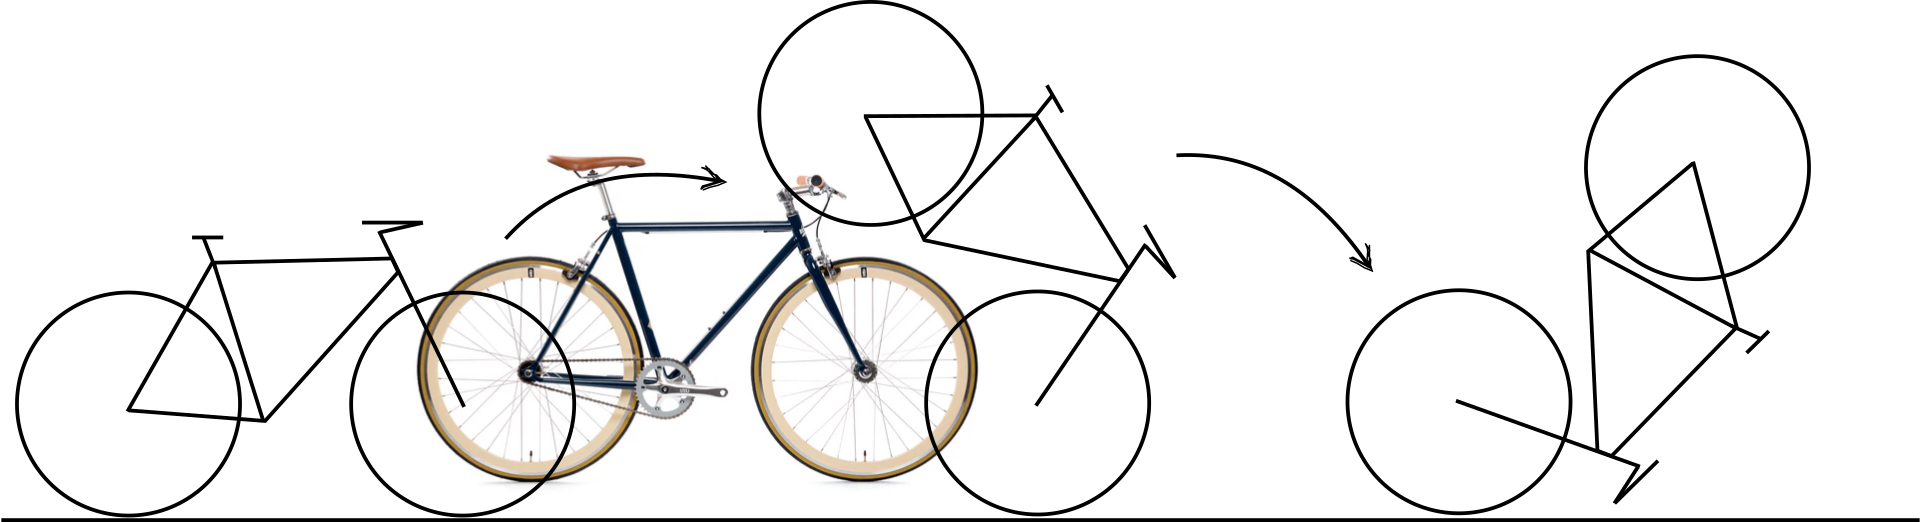
\includegraphics[width=\linewidth]{pitch-over.png}
%    \caption{Simple diagram of pitch-over motion.}
%    \label{fig: pitchover}
%\end{figure}

%\begin{figure}[h]
%    \centering
%    \includegraphics[width=\linewidth]{roll-over.png}
%    \caption{Simple diagram of roll-over motion.}
%    \label{fig: rollover}
%\end{figure}

%\begin{figure}[h]
%    \centering
%    \includegraphics[width=\linewidth]{high-side-draw.jpg}
%    \caption{Hand draw of a high-side crash.}
%    \label{fig: highside}
%\end{figure}




\section{Introduction}

This document aims to guide you to understand the proposed classification of single-cyclist crashes and label the samples sent to you.

\subsection{What is a single-cyclist crash?}

A single-cyclist crash is an event where the normal riding of the bicycle is disrupted and ends in a crash with no other road users involved.
%
Essentially, in this document will be assumed that a crash occurs when, during a manoeuvre, one or more excitations modify the state of the system in an unexpected way.
%
This excitation is the beginning of the `critical scenario', where we find the mechanisms that produce the crash.
%
Finally, the crash itself can be characterised by the motion of the bicycle and/or the rider in the outcome of the event.



\section{Bicycle dynamics-oriented classification}

The proposed workflow to classify the crash according to the observed characteristics is composed by four layers: manoeuvre, excitation of the system, mechanisms, and motion.
%
This multi-layer approach allows to classify the crash events with different depth levels according to the available information.
%


\subsection{Manoeuvre}

The first layer consists on the manoeuvre that the rider is executing at the moment of entering to the critical scenario.

\begin{itemize}
    \item \textbf{Straight-running:} The action of riding a straight path, maintaining balance through minor steering adjustments and no major variations on the states of the system.
    \item \textbf{Longitudinal acceleration:} Refers to braking and acceleration manoeuvres, both performed by the user.
    \item \textbf{Steady and planned cornering:} Refers to the situation where the rider is performing a controlled turning with a defined trajectory.
    \item \textbf{Low-speed:} Makes reference mainly to start and stop riding, where users require major steering control inputs to maintain the bicycle in upright position.
    \item \textbf{Unplanned turning or avoidance:} This is when the rider executes a sudden evasive turn or abrupt brake application to avoid an obstacle.
    \item \textbf{Stunt:} Refers to any action that is not explicitly required for normal riding, such as riding with one hand, no hands, or standing on the pedals, which limits the control of the rider on the bicycle.
\end{itemize}


\subsection{Excitation of the system}

For this research, the bicycle is assumed as an interface between the human and the environment.
%
Therefore, the bicycle is subjected to forces from the environment and from human control.
%
Additionally, the bicycle itself is a dynamic system which can present excitations in its motion, which are referred as intrinsic excitations.


\begin{itemize}
    \item \textbf{External excitations:} Mechanical forces that result from the interaction of the human-bicycle system with the environment.
    \item \textbf{Intrisic excitations:} Behaviour of the system due to its dynamical properties.
        %
        Its associated crash scenario is the excitation of a natural frequency of the system, creating an unstable and/or uncontrollable vehicle.
        %
        Possible mechanical failures on the bicycle also fit in this category.
    \item \textbf{Rider forces:} This makes reference to the control inputs from the human to the vehicle.
\end{itemize}



\subsection{Mechanisms of crash}

Here we detail mechanisms that make possible bicycle riding, however, in the analysis of crashes, we delve into the failure of these mechanisms.

\begin{itemize}
    \item \textbf{Modes of vibration:} These are the oscillatory modes of vibration of the bicycle: weave and wobble, creating an unpredictable trajectory of the bicycle.
        %
        Being the former a combination of roll and yaw angle, while the latter a high-frequency steering oscillation.
    \item \textbf{Rider-bicycle joint:} The rider is `attached' to the bicycle in five points: handlebar (both hands), pedals and saddle.
        %
        When one or more of these detaches, the rider loses a control input to the system.
    \item \textbf{Balance control:} This makes reference to the ability of the human to balance the bicycle as an inverted pendulum, moving the steering to control its equilibrium.
        %
        When the control action is not correct, the rider reaches a point where it is not possible to maintain the balance.
    \item \textbf{Load transfer:}  Longitudinal accelerations generate longitudinal load transfer, which remains unnoticed for most casual riders.
        %
        However, under large accelerations, this load transfer exceeds the maximum tolerable values for maintaining the bicycle in a stable configuration.
        %
        This can be caused by wrong control inputs on brake use, front collisions, objects stuck on the front wheel, etc.
    \item \textbf{Tyre friction:} The only connection between the bicycle and the environment is on the tyre-ground contact interface.
        %
        Tyres have a saturation limit for the grip offered, when this limit is reached, they start to skid and the rider loses control of the vehicle.
    \item \textbf{Contact forces:}  This makes reference to any collision or force exerted on the bicycle.
    \item \textbf{Aerodynamic forces:} Aerodynamic forces which are studied as a resultant in the centre of pressure of the system.
        %
        These can play an important role when large wind gusts strike the rider by the side, generating a major lateral force, which can destabilise the system.
\end{itemize}


\subsubsection{Notable remarks: control interfaces}

\begin{itemize}
    \item \textbf{Handlebar:} Through the handlebar the rider exerts steering torque to control the lateral balance of the bicycle.
    \item \textbf{Pedals:} In the pedals, the rider applies force to create the propulsion of the bicycle.
        %
        This interface is subjected to large forces when the system is in longitudinal acceleration.
    \item \textbf{Brakes:} To reduce the longitudinal speed of the system, the rider controls the brakes through handles.
        %
        If the control input is not precise, the system experiences excessive braking force, over its load transfer limits.
\end{itemize}


\subsection{Motion of the bicycle}

This is related to the main motion of the rear frame of the bicycle while the crash is occurring.
%
Due to the dynamics of the bicycle, and following the common simplification to its analysis, we find two main motions related to the degrees of freedom: pitch-over and roll-over.
%
Additionally, the roll-over motion includes its own sub-classification according to the direction of rotation with respect to the initial motion.
% 
Please visit  to watch an example of a crash where the roll angle is negative with respect to the intended turn.


\begin{itemize}
    \item \textbf{Pitch-over:} The main characteristic of this motion is one of the wheels lifting from the ground, following a trajectory that finishes with the front wheel behind the rear wheel (see Figure \ref{fig: pitchover}).
    \item \textbf{High-side:} Characterised for a sudden deceleration of the wheel while in lateral motion, which leads to a violent negative roll rate with respect to the direction of the initial motion (see Figure \ref{fig: highside}).
        %
        For an example visit \url{https://youtube.com/shorts/_etyqSpH10c?feature=shared}.
    \item \textbf{Low-side:} The human-bicycle system follows an excessive roll rate in the same direction as at the beginning (see Figure\ref{fig: lowside}).
    \item \textbf{No characteristic motion:} This sub-class refers to crashes where the final motion is not clear, or the main event is a collision that stops the motion.
\end{itemize}



\begin{figure}
    \centering
    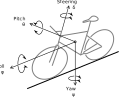
\includegraphics[scale=1.0]{bike-dof.png}
    \caption{Rotation axes of the bicycle.}
    \label{fig: bike-dof}
\end{figure}


\begin{figure}
    \centering
    \begin{subfigure}[t]{0.3\textwidth}
        \centering
        \includegraphics[width=\textwidth]{pitch-over-stage1.png}
        \caption{Normal riding.}
    \end{subfigure}%
    \begin{subfigure}[t]{0.3\textwidth}
        \centering
        \includegraphics[width=\textwidth]{pitch-over-stage2.png}
        \caption{Deceleration generates load transfer that exceeds rear normal force and the rotation motion starts around the contact point of the front wheel.}
    \end{subfigure}
    \begin{subfigure}[t]{0.3\textwidth}
        \centering
        \includegraphics[width=\textwidth]{pitch-over-stage3.png}
        \caption{The rotational inertia of the system produces a complete rotation of the system.}
    \end{subfigure}
    \caption{Pitch-over crash sequence.}
    \label{fig: pitchover}
\end{figure}

\begin{figure}
    \centering
    \includegraphics[width=1.0\linewidth]{high-side-v2.eps}
    \caption{Schematic representation of a high-side crash.}
    \label{fig: highside}
\end{figure}

\begin{figure}
    \centering
    
\includegraphics[width=1.0\linewidth]{low-side-v2.eps}
    \caption{Schematic representation of a low-side crash.}
    \label{fig: lowside}
\end{figure}

\section{Example}

Let's do an example using the following video \url{https://youtube.com/shorts/VZibdrdhdgM?feature=shared}.


First, in the moment of the crash, it is observed that the rider is performing a planned turn into the left-hand corner.
%
Then, it is observed that the steering angle increases at mid corner, which could be the result of traction loss in the front wheel.
%
Finally, the fall motion of the rider is a roll-over low-side, because the roll angle increases in the same direction than the initial motion.


Since there are no visible failure mechanisms on the bicycle, and the rider seems to have controlled the bicycle in the proper way, it is assumed that the excitation is merely external.
%
This refers to a tyre friction mechanism, where the front tyre appears to have reached its saturation limit on the lateral load.
%
Therefore, the bicycle presents an understeering behaviour, the trajectory of the front wheel changes, and the cornering equilibrium dissapears.


Thus, this crash is a front-skidding low-side.



\section{Closing words}

This classification aims to provide a wide coverage of bicycle crashes, taking into account factors, mechanisms and common motions.
%
However, it is still possible that with the available information, the event does not fit properly in the available options.
%
For this reason, this work allows to classify crashes with a combination of different layers and multiple choices by category.



\begin{thebibliography}{9}

    \bibitem{Jac04} Elin K. Jacob (2004):  Classification and Categorization: A Difference that makes a Difference. Graduate School of Library and Information Science. University of Illinois at Urbana-Champaign. \url{http://hdl.handle.net/2142/1686}

    \bibitem{Moo12} Moore, Jason (2012): Human Control of a Bicycle. Doctoral thesis, University of California Davis.


\end{thebibliography}


\end{document}
